\documentclass[12pt]{article}
\usepackage{lecture}
\usepackage{html}
\usepackage{url}
\usepackage{graphics}
\usepackage{epstopdf}

\newcommand{\copyrightYears}{2001-2015}

\title{The Genetics of Natural Selection}

\begin{document}

\maketitle

\thispagestyle{first}

\section*{Introduction}

So far in this course, we've focused on describing the pattern of
variation within and among populations. We've talked about inbreeding,
which causes {\it genotype\/} frequencies to change, although it
leaves allele frequencies the same, and we've talked about how to
describe variation among populations. But we haven't yet discussed any
evolutionary processes that could lead to a change in allele
frequencies within populations.\footnote{We mentioned migration and
  drift in passing, and I'm sure you all understand the rudiments of
  them, but we haven't yet discussed them in detail.}

Let's return for a moment to the list of assumptions we developed when
we derived the Hardy-Weinberg principle and see what we've done so
far.

\begin{description}

\item[Assumption \#1] Genotype frequencies are the same in males and
females, e.g., $x_{11}$ is the frequency of the $A_1A_1$ genotype in
both males and females.

\item[Assumption \#2] Genotypes mate at random {\it with respect to
their genotype at this particular locus}.

\item[Assumption \#3] Meiosis is fair. More specifically, we assume
that there is no segregation distortion, no gamete competition, no
differences in the developmental ability of eggs, or the fertilization
ability of sperm.

\item[Assumption \#4] There is no input of new genetic material, i.e.,
gametes are produced without mutation, and all offspring are produced
from the union of gametes within this population.

\item[Assumption \#5] The population is of infinite size so that the
actual frequency of matings is equal to their expected frequency and
the actual frequency of offspring from each mating is equal to the
Mendelian expectations.

\item[Assumption \#6] All matings produce the same number of
offspring, on average.

\item[Assumption \#7] Generations do not overlap.

\item[Assumption \#8] There are no differences among genotypes in the
probability of survival.

\end{description}

The only assumption we've violated so far is Assumption \#2, the
random-mating assumption. We're going to spend the next several
lectures talking about what happens when you violate Assumptions \#3,
\#6, and \#8. When any one of those assumptions is violated we have
some form of natural selection going on.\footnote{As I alluded to when
  we first started talking about inbreeding, we can also have natural
  selection as a result of certain types of violations of assumption
  \#2, e.g., sexual selection or disassortative mating. See
  below.}\index{natural selection}

\subsection*{Components of selection}

Depending on which of those three assumptions is violated and how it's
violated we recognize that selection may happen in different ways and
at different life-cycle stages.\footnote{To keep things {\it
    relatively\/} simple we're not even going to discuss differences
  in fitness that may be associated with different ages. We'll assume
  a really simple life-cycle in which there are non-overlapping
  generations. So we don't need to distinguish between fitness
  components that differ among age categories.}\index{components of
  selection}\index{natural selection!components of selection}

\begin{description}

\item[Assumption \#3:] {\it Meiosis is fair}. There are at least two
  ways in which this assumption may be violated.

\begin{itemize}

\item {\it Segregation distortion\/}: The two alleles are not equally
  frequent in gametes produced by heterozygotes. The $t$-allele in
  house mice, for example, is found in 95\% of fertile sperm produced
  by heterozygous males.\index{segregation distortion}\index{natural selection!segregation distortion}

\item {\it Gamete competition\/}: Gametes may be produced in equal
  frequency in heterozygotes, but there may be competition among them
  to produce fertilized zygotes, e.g., sperm competition in animals,
  pollen competition in seed plants.\index{gamete
    competition}\index{natural selection!gamete competition}\footnote{Strictly speaking pollen competition isn't
    gamete competition, although the evolutionary dynamics are the
    same. I'll leave it to the botanists among you to explain to the
    zoologists why pollen competition would be more properly called
    {\it gametophytic\/} competition.}

\end{itemize}

\item[Assumption \#6:] {\it All matings produce the same number of
progeny.}

\begin{itemize}

\item {\it Fertility selection\/}: The number of offspring produced
  may depend on maternal genotype ({\it fecundity selection\/}),
  paternal genotype ({\it virility selection\/}), or on
  both.\index{fertility selection}\index{fecundity selection}\index{virility selection}\index{natural selection!fertility selection}

\end{itemize}

\item[Assumption \#8:] {\it Survival does not depend on genotype.}

\begin{itemize}

\item {\it Viability selection\/}: The probability of survival from
  zygote to adult may depend on genotype, and it may differ between
  sexes.\index{viability selection}\index{natural selection!viability
    selection}

\end{itemize}

\end{description}

At this point you're probably thinking that I've covered all the
possibilities. But by now you should also know me well enough to guess
from the way I wrote that last sentence that if that's what you were
thinking, you'd be wrong. There's one more way in which selection can
happen that corresponds to violating

\begin{description}

\item[Asssumption \#2:] {\it Individuals mate at random.}

\begin{itemize}

\item {\it Sexual selection\/}: Some individuals may be more
  successful at finding mates than others. Since females are typically
  the limiting sex (Bateman's principle), the differences typically
  arise either as a result of {\it male-male competition\/} or {\it
    female choice}.\index{sexual selection}\index{natural selection!sexual selection}

\item {\it Disassortative mating\/}: When individuals preferentially
  choose mates different from themselves, rare genotypes are favored
  relative to common genotypes. This leads to a form a
  frequency-dependent selection.\index{disassortative mating}\index{natural selection!disassortative mating}

\end{itemize}

\end{description}

\section*{The genetics of viability selection}

That's a pretty exhaustive (and exhausting) list of the ways in which
selection can happen. Although we're going to focus our study of
natural selection just on viability selection, it's important to
remember that any or all of the other forms of selection may be
operating simultaneously on the genes or the traits that we're
studying, and the direction of selection due to these other components
may be the same or different as the direction of viability
selection. We're going to focus on viability selection for two
reasons:\index{viability selection!genetics}

\begin{enumerate}

\item The most basic properties of natural selection acting on other
  components of the life history are similar to those of viability
  selection. A good understanding of viability selection provides a
  solid foundation for understanding other types of
  selection.\footnote{There are some important differences, however,
    and I hope we have time to discuss a couple of them.}

\item The algebra associated with understanding viability selection is
  a {\it lot\/} simpler than the algebra associated with understanding
  the other types of selection, and the dynamics are simpler and
  easier to understand.\footnote{Once you've seen what you're in for
    you may think I've lied about this. But if you really think I
    have, just ask me to illustrate some of the algebra necessary for
    understanding viability selection when males and females differ in
    fitness. That's about as simple an extension as you can imagine,
    and things start to get pretty complicated even then.}

\end{enumerate}

\subsection*{The basic framework}

To understand the basics, we'll start with a numerical example using
some data on {\it Drosophila pseudoobscura\/} that Theodosius
Dobzhansky collected more than 50 years ago. You may remember that
this species has chromosome inversion polymorphisms. Although these
inversions involve many genes, they are inherited as if they were
single Mendelian loci, so we can treat the karyotypes as single-locus
genotypes and study their evolutionary dynamics. We'll be considering
two inversion types the Standard inversion type, $ST$, and the
Chiricahua inversion type, $CH$. We'll use the following notation
throughout our discussion:\index{Drosophila@\textit{Drosophila}!\textit{pseudoobscura}}

\begin{center}
\begin{tabular}{cc}
\hline\hline
Symbol  & Definition \\
\hline
$N$      & number of individuals in the population \\
$x_{11}$ & frequency of $ST/ST$ genotype \\
$x_{12}$ & frequency of $ST/CH$ genotype \\
$x_{22}$ & frequency of $CH/CH$ genotype \\
$w_{11}$ & fitness of $ST/ST$ genotype, probability of surviving from
           egg to adult \\
$w_{12}$ & fitness of $ST/CH$ genotype \\
$w_{22}$ & fitness of $CH/CH$ genotype \\
\hline
\end{tabular}
\end{center}

The data look like this:\footnote{Don't worry for the moment about how
the viabilities were estimated.}

\begin{center}
\begin{tabular}{l|ccc}
\hline\hline
Genotype         & $ST/ST$    & $ST/CH$    & $CH/CH$    \\
\hline
Number in eggs   & 41       & 82       & 27       \\
                 & $x_{11}N$  & $x_{12}N$  & $x_{22}N$  \\
viability        & 0.6      & 0.9      & 0.45     \\
                 & $w_{11}$   & $w_{12}$   & $w_{22}$   \\
Number in adults & 25       & 74       & 12       \\
                 & $w_{11}x_{11}N$ & $w_{12}x_{12}N$ & $w_{22}x_{22}N$ \\
\hline
\end{tabular}
\end{center}

\section*{Genotype and allele frequencies}

It should be trivial for you by this time to calculate the genotype
frequencies in eggs and adults. We'll be using the convention that
genotype frequencies in eggs (or newly-formed zygotes) are the
genotype frequencies {\it before selection\/} and that genotype
frequencies in adults are the genotype frequencies {\it after
  selection}.

\begin{eqnarray*}
\mbox{freq($ST/ST$) before selection}
 &=& \frac{41}{41 + 82 + 27} \\
 &=& 0.27 \\
\mbox{freq($ST/ST$) before selection}
 &=& \frac{Nx_{11}}{Nx_{11} + Nx_{12} + Nx_{22}} \\
 &=& x_{11} \\
 && \\
\mbox{freq($ST/ST$) after selection}
 &=& \frac{25}{25 + 74 +12} \\
 &=& 0.23 \\
\mbox{freq($ST/ST$) after selection}
 &=& \frac{w_{11}x_{11}N}{w_{11}x_{11}N + w_{12}x_{12}N + w_{22}x_{22}N} \\
 &=& \frac{w_{11}x_{11}}{w_{11}x_{11} + w_{12}x_{12} +
 w_{22}x_{22}} \\
 &=& \frac{w_{11}x_{11}}{\bar w} \\
 \bar w &=& \frac{w_{11}x_{11}N + w_{12}x_{12}N + w_{22}x_{22}N}{N} \\
        &=& w_{11}x_{11} + w_{12}x_{12} + w_{22}x_{22} \quad ,
\end{eqnarray*}
where $\bar w$ is the mean fitness, i.e., the average probability of
survival in the population.\index{mean fitness}

It is also trivial to calculate the allele frequencies before and
after selection:

\begin{eqnarray*}
\hbox{freq($ST$) before selection}
 &=& \frac{2(41) + 82}{2(41 + 82 + 27)} \\
 &=& 0.55 \\
\hbox{freq($ST$) before selection}
 &=& \frac{2(Nx_{11}) + Nx_{12}}{2(Nx_{11} + Nx_{12} + Nx_{22})} \\
 &=& x_{11} + x_{12}/2 \\
&& \\
\hbox{freq($ST$) after selection}
 &=& \frac{2(25) + 74}{2(25 + 74 + 12)} \\
 &=& 0.56 \\
\hbox{freq($ST$) after selection}
 &=& \frac{2w_{11}x_{11}N + w_{12}x_{12}N}{2(w_{11}x_{11}N + w_{12}x_{12}N + w_{22}x_{22}N)} \\
 &=& \frac{2w_{11}x_{11} + w_{12}x_{12}}{2(w_{11}x_{11} + w_{12}x_{12} + w_{22}x_{22})} \\
p' &=& \frac{w_{11}x_{11} + w_{12}x_{12}/2}{w_{11}x_{11} +
 w_{12}x_{12} + w_{22}x_{22}} \\
x_{11} &=& p^2, \quad x_{12} = 2pq, \quad x_{22} = q^2 \\
p' &=& \frac{w_{11}p^2 + w_{12}pq}{w_{11}p^2 + w_{12}2pq + w_{22}q^2} \\
\bar w &=& w_{11}x_{11} + w_{12}x_{12} + w_{22}x_{22} \\
       &=& p^2w_{11} + 2pqw_{12} + q^2w_{22}
\end{eqnarray*}

If you're still awake, you're probably wondering\footnote{Okay,
  ``probably'' is an overstatement. ``May be'' would have been a
  better guess.} why I was able to substitute $p^2$, $2pq$, and $q^2$
for $x_{11}$, $x_{12}$, and $x_{22}$. Remember what I said earlier
about what we're doing here. The {\it only\/} Hardy-Weinberg
assumption we're violating is the one saying that all genotypes are
equally likely to survive from zygote to adult. Remember also that a
single generation in which all of the conditions for Hardy-Weinberg is
enough to establish the Hardy-Weinberg proportions. Putting those two
observations together, it's not too hard to see that genotypes will be
in Hardy-Weinberg proportions in newly formed zygotes. Viability
selection will change that later in the life-cycle, but we restart
every generation with genotypes in the familiar Hardy-Weinberg
proportions, $p^2$, $2pq$, and $q^2$, where $p$ is the frequency of
$ST$ in the {\it parental\/} generation.\index{selection equation}

\subsection*{Selection acts on relative viability}

Let's stare at the selection equation for awhile and see what it
means.
\begin{equation}
p' = \frac{w_{11}p^2 + w_{12}pq}{\bar w} \quad . \label{eq:absolute}
\end{equation}
Suppose, for example, that we were to divide the numerator and
denominator of~(\ref{eq:absolute}) by $w_{11}$.\footnote{I'm dividing
  by 1, in case you hadn't noticed.} We'd then have
\begin{equation}
p' = \frac{p^2 + (w_{12}/w_{11})pq}{(\bar w/w_{11})} \quad . \label{eq:relative}
\end{equation}
Why did I bother to do that? Well, notice that we start with the same
allele frequency, $p$, in the parental generation in both equations
and that we end up with the same allele frequency in the offspring
generation, $p'$, in both equations, but the fitnesses are different:
\begin{center}
\begin{tabular}{c|ccc}
\hline\hline
         & \multicolumn{3}{c}{Fitnesses} \\
Equation & $A_1A_1$ & $A_1A_2$ & $A_2A_2$ \\
\hline
\ref{eq:absolute} & $w_{11}$ & $w_{12}$ & $w_{22}$ \\
\ref{eq:relative} & 1 & $w_{12}/w_{11}$ & $w_{22}/w_{11}$ \\
\hline
\end{tabular}
\end{center}
I could have, of course, divided the numerator and denominator by
$w_{12}$ or $w_{22}$ intead and ended up with yet other sets of
fitnesses that produce exactly the same change in allele
frequency. This illustrates the following general principle:
\begin{quote}
The consequences of natural selection (in an infinite population)
depend only on the {\it relative\/} magnitude of fitnesses, not on
their {\it absolute\/} magnitude.\index{relative fitness}
\end{quote}
That means, for example, that in order to predict the outcome of
viability selection, we don't have to know the probability that each
genotype will survive, their {\it absolute viabilities}. We only need
to know the probability that each genotype will survive relative to
the probability that other genotypes will survive, their {\it relative
  viabilities}. As we'll see later, it's sometimes easier to estimate
the relative viabilities than to estimate absolute
viabilities.\footnote{We'll also see when we get to studying the
  interaction between natural selection and drift that this statement
  is no longer true. To understand how drift and selection interact we
  have to know something about {\it absolute\/} viabilities.}\index{viability!absolute}\index{viability!relative}

\subsection*{Marginal fitnesses}

In case you haven't already noticed, there's almost always more than
one way to write an equation.\footnote{And you won't have noticed this
  and may not believe me when I tell you, but I'm {\it not\/} showing
  you every possible way to write these equations.} They're all
mathematically equivalent, but they emphasize different things. In
this case, it can be instructive to look at the difference in allele
frequencies from one generation to the next, $\Delta p$:
\begin{eqnarray*}
\Delta p &=& p' - p \\
&=& \frac{w_{11}p^2 + w_{12}pq}{\bar w} - p \\
&=& \frac{w_{11}p^2 + w_{12}pq - \bar wp}{\bar w} \\
&=& \frac{p(w_{11}p + w_{12}q - \bar w)}{\bar w} \\
&=& \frac{p(w_1 - \bar w)}{\bar w} \quad ,
\end{eqnarray*}
where $w_1$ is the {\it marginal fitness\/} of allele $A_1$. To
explain why it's called a {\it marginal\/} fitness, I'd have to teach
you some probability theory that you probably don't want to
learn.\footnote{But remember this definition of marginal viability
anyway. You'll see it return in a few weeks when we talk about the
additive effect of an allele and about Fisher's Fundamental Theorem of
Natural Selection.} Fortunately, all you really need to know is that
it corresponds to the probability that a randomly chosen $A_1$ allele
in a newly formed zygote will survive into a reproductive
adult.\index{marginal fitness}

Why do we care? Because it provides some (obvious) intuition on how
allele frequencies will change from one generation to the next. If
$w_1 > \bar w$, i.e., if the chances of a zygote carrying an $A_1$
allele of surviving to make an adult are greater than the chances of a
randomly chosen zygote, then $A_1$ will increase in frequency. If $w_1
< \bar w$, $A_1$ will decrease in frequency. Only if $p=0$, $p=1$, or
$w_1=\bar w$ will the allele frequency not change from one generation
to the next.

\section*{Patterns of natural selection}

Well, all that algebra was lots of fun,\footnote{I'm kidding, in case
  you couldn't tell.} but what good did it do us? Not an enormous
amount, except that it shows us~(not surprisingly), that allele
frequencies are likely to change as a result of viability selection,
and it gives us a nice little formula we could plug into a computer to
figure out exactly how. One of the reasons that it's
useful\footnote{If not exactly fun.} to go through all of that algebra
is that it's possible to make predictions about the consequences of
natural selection simply by knowing the pattern of viaiblity
differences. What do I mean by pattern? Funny you should
ask~(Table~\ref{table:patterns}).\index{natural selection!patterns}

\begin{table}
\begin{center}
\begin{tabular}{ccc}
\hline\hline
Pattern & Description & Figure \\
\hline
Directional & $w_{11} > w_{12} > w_{22}$ & Figure~\ref{fig:directional} \\
            & or \\
            & $w_{11} < w_{12} < w_{22}$ & \\
Disruptive  & $w_{11} > w_{12}$, $w_{22} > w_{12}$
                                         & Figure~\ref{fig:disruptive} \\
Stabiliizing& $w_{11} < w_{12}$, $w_{22} < w_{12}$
                                         & Figure~\ref{fig:stabilizing} \\
\hline
\end{tabular}
\end{center}
\caption{Patterns of viability selection at one locus with two alleles.}\label{table:patterns}
\end{table}

Before exploring the consequences of these different patterns of
natural selection, I need to introduce you to a very important result:
Fisher's Fundamental Theorem of Natural Selection. We'll go through
the details later when we get to quantitative genetics. For now all
you need to know is that viability selection causes the mean fitness
of the progeny generation to be greater than or equal to the mean
fitness of the parental generation, with equality only at equilibrium,
i.e.,
\[
\bar w' \ge \bar w \quad .
\]
How does this help us? Well, the best way to understand that is to
illustrate how we can use Fisher's theorem to predict the outcome of
natural selection when we know only the pattern of viability
differences. Let's take each pattern in turn.\index{Fisher's Fundamental Theorem of Natural Selection}

\subsection*{Directional selection}

To use the Fundamental Theorem we plot $\bar w$ as a function of
$p$~(Figure~\ref{fig:wbar}(a) and~\ref{fig:wbar}(b)). The Fundamental
Theorem now tells us that allele frequencies have to change from one
generation to the next in such a way that $\bar w' > \bar w$, which
can only happen if $p' > p$. So viability selection will cause the
frequency of the $A_1$ allele to increase in panel (a) and decrease in
panel (b).\index{directional selection}\index{selection!directional
  selection} Ultimately, the population will be monomorphic for the
homozygous genotype with the highest fitness.\footnote{A population is
  {\it monomorphic\/} at a particular locus when only one allele is
  present. If a population is monomorphic for allele $A_1$, I might
  also say that allele $A_1$ is fixed in the population or that the
  population is fixed for allele
  $A_1$.\index{monomorphic}\index{allele fixation}}

\begin{figure}
\begin{center}
\resizebox{!}{6in}{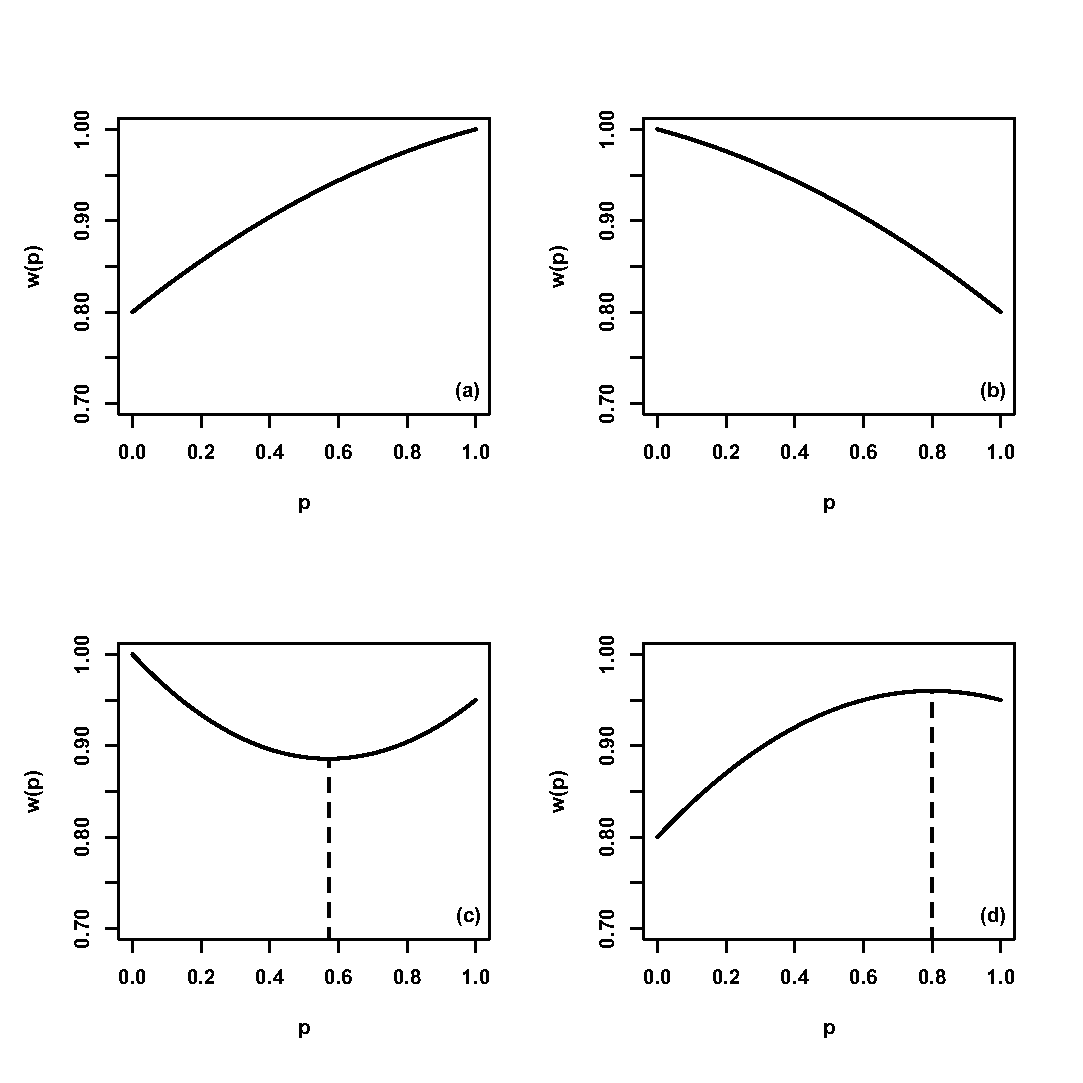
\includegraphics{wbar.eps}}
\end{center}
\caption{With {\it directional selection\/} (panel (a) $w_{11} > w_{12} >
w_{22}$, panel (b) $w_{11} > w_{12} > w_{22}$) viability selection
leads to an ever increasing frequency of
the favored allele.  Ultimately, the population will be monomorphic
for the homozygous genotype with the highest
fitness. With {\it disruptive selection\/} (panel (c) $w_{11} >
w_{12}$ and $w_{22} > w_{12}$) viability selection may lead either to
an increasing   frequency of the $A$ allele or to a decreasing frequency.
  Ultimately, the population will be monomorphic for one of the
  homozygous genotypes.  Which homozygous genotype comes to
  predominate, however, depends on the initial allele frequencies in
  the population. With {\it stabilizing selection\/} (panel (d) $w_{11} < w_{12}
  > w_{22}$; also called balancing selection or heterozygote
  advantage) viability selection will lead to a stable polymorphism.
  All three genotypes will be present at equilibrium.}\label{fig:wbar}
\end{figure}

\subsection*{Disruptive selection}

If we plot $\bar w$ as a function of $p$ when $w_{11} > w_{12}$ and
$w_{22} > w_{12}$, we wee a very different
pattern~(Figure~\ref{fig:wbar}(c)). Since the Fundamental Theorem
tells us that $\bar w' \ge \bar w$, we know that if the population
starts with an allele on one side of the bowl $A_1$, will be lost. If
it starts on the other side of the bowl, $A_2$ will be
lost.\footnote{Strictly speaking, we need to know more than $\bar w'
  \ge \bar w$, but we do know the other things we need to know in this
  case. Trust me. Have I ever lied to you? (Don't answer
  that.)}\index{disruptive selection}\index{selection!disruptive}

Let's explore this example a little further. To do so, I'm going to
set $w_{11} = 1 + s_1$, $w_{12} = 1$, and $w_{22} = 1+
s_2$.\footnote{Why can I get away with this? Hint: Think about
  relative fitnesses.} When fitnesses are written this way $s_1$ and
$s_2$ are referred to as {\it selection coefficients}. Notice also
with these definitions that the fitnesses of the homozygotes are
greater than 1.\footnote{Which is why I gave you the relative fitness
  hint in the last footnote.} Using these definitions and plugging
them into~(\ref{eq:absolute}),\index{selection coefficient}
\begin{eqnarray}
p' &=& \frac{p^2(1+s_1) + pq}{p^2(1+s_1) + 2pq + q^2(1+s_2)} \nonumber
   \\
   &=& \frac{p(1 + s_1p)}{1 + p^2s_1 + q^2s_2} \quad . \label{eq:disruptive}
\end{eqnarray}
We can use equation~(\ref{eq:disruptive}) to find the equilibria of
this system, i.e., the values of $p$ such that $p' = p$.\index{equilibrium}
\begin{eqnarray*}
p &=& \frac{p(1 + s_1p)}{1 + p^2s_1 + q^2s_2} \\
p(1 + p^2s_1 + q^2s_2) &=& p(1 + s_1p) \\
p\left((1 + p^2s_1 + q^2s_2) - (1 + s_1p)\right) &=& 0 \\
p\left(ps_1(p - 1) + q^2s_2\right) &=& 0 \\
p(-pqs_1 + q^2s_2) &=& 0 \\
pq(-ps_q + qs_2) &=& 0 \quad .
\end{eqnarray*}
So $p'=p$ if $\hat p=0$, $\hat q=0$, or $\hat ps_1 = \hat
qs_2$.\footnote{Remember that the ``hats'' can mean either the
  estimate of an unknown paramter or an equilibrium. The context will
  normally make it clear which meaning applies. In this case it should
  be pretty obvious that I'm talking about equilibria.} We can
simplify that last one a little further, too.
\begin{eqnarray*}
\hat ps_1 &=& \hat qs_2 \\
\hat ps_1 &=& (1-\hat p)s_2 \\
\hat p(s_1 + s_2) &=& s_2 \\
\hat p &=& \frac{s_2}{s_1+s_2} \quad .
\end{eqnarray*}

Fisher's Fundamental Theorem tells us which of these equilibria
matter. I've already mentioned that depending on which side of the
bowl you start, you'll either lose the $A_1$ allele or the $A_2$
allele. But suppose you happen to start {\it exactly\/} at the bottom
of the bowl. That corresponds to the equilibrium with $\hat p =
s_2/(s_1+s_2)$. What happens then?

Well, if you start {\it exactly\/} there, you'll stay there forever
(in an infinite population). But if you start ever so slightly off the
equilibrium, you'll move farther and farther away. It's what
mathematicians call an {\it unstable equilibrium}. Any departure from
that equilibrium gets larger and larger. For evolutionary purposes, we
don't have to worry about a population getting to an unstable
equilibrium. It never will. Unstable equilibria are ones that
populations evolve away from.\index{equilibrium!unstable}

When a population has only one allele present it is said to be {\it
  fixed\/} for that allele. Since having only one allele is also an
equilibrium (in the absence of mutation), we can also call it a {\it
  monomorphic equilibrium}. When a population has more than one allele
present, it is said to be {\it polymoprhic}. If two or more alleles
are present at an equilibrium, we can call it a {\it polymorphic
  equilibrium}. Thus, another way to describe the results of
disruptive selection is to say that the monomorphic equilibria are
stable, but the polymorphic equilibrium is not.\footnote{Notice that a
  polymorphic equilibrium doesn't even exist when selection is
  directional.}\index{allele fixation}\index{equilibrium!monomorphic}\index{equilibrium!polymorphic}

\subsection*{Stabilizing selection}

If we plot $\bar w$ as a function of $p$ when $w_{11} < w_{12}$ and
$w_{22} < w_{12}$, we see a third pattern. The plot is shaped like an
upside down bowl~(Figure~\ref{fig:wbar}).\index{stabilizing selection}\index{selection!stabilizing}

In this case we can see that no matter what allele frequency the
population starts with, the only way that $\bar w' \ge \bar w$ can
hold is if the allele frequency changes in such a way that it gets
close to the value where $\bar w$ is maximized every
generation. Unlike directional selection or disruptive selection, in
which natural selection tends to eliminate one allele or the other,
stabilizing selection tends to keep both alleles in the
population. You'll also see this pattern of selection referred to as
balancing selection, because the selection on each allele is
``balanced'' at the polymorphic equilibria.\footnote{In fact, the
  marginal fitnesses are equal, i.e., $w_1=w_2$.} We can summarize the
results by saying that the monomorphic equilibria are unstable and
that the polymorphic equilibrium is stable. By the way, if we write
the fitness as $w_{11} = 1 - s_1$, $w_{12}=1$, and $w_{22}=1-s_2$,
then the allele frequency at the polymorphic equilibrium is $\hat
p=s_2/(s_1+s_2)$.\footnote{I'm not showing the algebra that justifies
  this conclusion on the off chance that you may want to test your
  understanding by verifying it yourself.}

\end{document}
